\documentclass[a4paper,11pt]{article}
\usepackage{amssymb}
\usepackage{mathbbold}
\usepackage{latexsym}
\usepackage{amsmath}
\usepackage{url}
\usepackage{graphicx}
\usepackage{amsthm}
\parindent=0in
\author{Bi Ran(U087272L)}
\title{Hand Written Digit Recognition and Its Improvement}
\frenchspacing

\begin{document}
\maketitle
\begin{abstract}
In this paper, three algorithms(C4.5, SVM) are compared on the task of handwritten digits recognition. Result shows that pairwise C4.5 and boosted C4.5 performance much better than C4.5 itself, while SVM gives the best performance. A feature extracting method is proposed, which aims to improve classification performance by extract useful features manually. It is shown that performance of C4.5 and SVM has significant improvement on data set with new features added.
\end{abstract}
\section{Introduction}
 Handwritten digits recognition is a classic problem of machine learning. The objective is to recognize images of isolated handwritten digits(0-9). More specifically, the problem is equivalent to look for a model, which takes image of handwritten digit as input, and output the predicted class label of the image, which is a digit from 0 to 9. The objective is to find a model which makes prediction with high accuracy. In practice, different writing style, bad handwriting and ambiguity among similar shaped digits make some images hard to recognize.
 
 The first part of the paper compares the performance between C4.5, its variation: pairwise C4.5, boosting and SVM algorithms. Parameter search is applied to achieve relatively good performance for C4.5 and SVM. Semeion Handwritten Digit Data Set is used for training and testing in this paper. Considering the limited size of data set, cross-validation is used for performance evaluation. The second part introduces a method to improve classification performance by applying feature extraction. Extracted features are appended to the original data set. It will also be shown that the feature extraction method generalize well on another handwritten digit data set(MNIST).
\section{Background and Motivation}
Handwritten digit recognition has important usage such as recognizing zip code and online recognition on computer tablets. Algorithms like support vector machine and neural network are commonly applied to solve this problem. Convolutional neural network has error rate less than 1\% on MNIST data set\cite{lecun98}. \\
In some cases, ``reject'' is allowed when doing classification. For example, in case of post code recognition, if the post code of some letter is hard to recognize, then the letter can be rejected, and will be send back to the sender. Sometimes, reject is preferred compared to misclassification. Foe example, in the same case of post code recognition, sending the letter back to the sender is much cheaper than sending it to a wrong place. Neural network has been applied on this situation, and the preference of ``reject'' or ``misclassification'' can be controlled by tunable threshold\cite{slg92}. In this paper, we do not consider ``reject'' case, and the target is simply maximize the accuracy of classification.\\
Decision tree is popular in data mining, while it is rarely used to do handwriting recognition in practice. SVM is a relatively new algorithm in machine learning, and it is one the algorithm which is comparable to Convolutional neural network on MNIST data set\cite{lecun98}. It is interesting to study why decision tree does not work well in handwritten digit recognition, while SVM has good performance. Testing various method to improve performance of decision tree may help discover some new potential of this old algorithm.
\section{Data set}
Semeion Handwritten Digit Data Set(\url{http://archive.ics.uci.edu/ml/datasets/Semeion+Handwritten+Digit}) is used for training and testing in this paper. 1593 handwritten digits from around 80 persons were scanned. Each digit stretched in a rectangular box 16x16 in a gray scale of 256 values.Then each pixel of each image was scaled into a 0-1 value using a fixed threshold. Thus each instance in the data set consists of 256 0-1 value, and a class label(0-9).\\
Each person wrote on a paper all the digits from 0 to 9, twice. The commitment was to write the digit the first time in the normal way (Figure 1) and the second time in a fast way (Figure 2). \\
The order of the examples in the data set is shuffled before training and testing, because the label distribution of the original data set is not random.
\begin{figure}
\centering
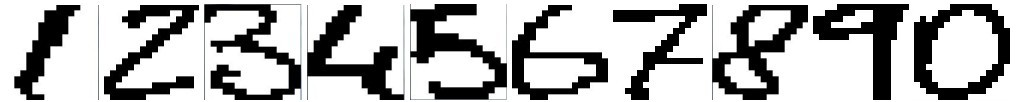
\includegraphics[width=1.0\textwidth]{clear}
\caption{written in normal way}
\end{figure}

\begin{figure}
\centering
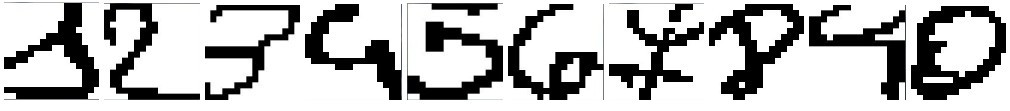
\includegraphics[width=1.0\textwidth]{unclear}
\caption{written in fast way}
\end{figure}

\section{Evaluation}

Because of the limited size of data set, we apply cross validation for evaluation purpose. Considering the trade-off between accuracy of estimation and time cost, we use 10-folds cross validation for performance evaluation, and compare the error rates of different algorithms.\\
In this paper, \emph{WEKA}(\url{http://www.cs.waikato.ac.nz/ml/weka/}) is used for all experiments of C4.5. \emph{LIBSVM}\cite{libsvm} is used for training and testing SVM.\\
\section{Experiment}
\subsection{C4.5}
Decision tree is a popular algorithm in data mining and machine learning. There are many decision tree algorithms. We only consider C4.5 in this paper. C4.5 is an improved version of ID3 decision tree. It follows a simple inductive bias: ``smaller trees are preferred'', which is motivated by Occan's Razor principle.\\
To further simplify the decision tree to avoid over fitting problem, C4.5 perform pruning to limit the size of the tree. To achieve good performance, we perform parameter search on two tunable parameters: $C$ and $minObj$. $C$ is confident factor, which is a probability threshold of the probability of the actual error rate being worse than the pessimistic estimation\cite{morgan.kaufmann}. A pessimistic estimation of the error rate for each subtree is used when do the subtree replacement and subtree raising pruning in C4.5 algorithm. Smaller confidence factor implies more pessimistic estimation, which will cause more drastic pruning. The $minObj$ is the minimum number of instances each leaf could have. Larger $minObj$ leads to smaller trees, which makes the tree more robust to noise.
\vspace{0.5cm}\\
\begin{tabular}{c|c c c c}
C$\backslash$ minObj	&1		&2		&3		&4\\
\hline \hline
1e-3 	&24.6077 \%	&24.3566 \%	&24.1682 \%	 &24.6704 \%\\
1e-2	&24.4193 \%	 &24.4821 \%	&24.231  \%	 &24.5449 \%\\
1e-1	&24.6077 \%	&24.231  \%	&24.231  \%	 &24.6077 \%\\
0.5 &24.2938 \%     &24.0427 \% &24.1055 \%  &24.8588 \%\\
1	&24.6077 \%	    &23.7916 \%	&24.1682 \%	 &24.796  \%\\
\end{tabular}
\vspace{0.5cm}\\
The result in the table above shows that he error rate of C4.5 algorithm is lowest(23.7916\%) when $C=1$ and $minObj=2$. The result shows that changing parameter has little influence on performance. This implies that pruning does not help much in this data set.\\
This result is very poor compared to many other popular algorithms like support vector machine(will see it later). There are some possible reasons:\\
\begin{enumerate}
\item[1] Decision tree algorithm itself has limitation. The problem of learning optimal decision tree is NP-complete\cite{dtnpc}, and C4.5 use a greedy algorithm, which does not guarantee to find the optimal decision tree.
\item[2] Although decision tree is able to estimate any discrete functions, some functions are harder to learn than others for decision trees. e.g. OXR function is hard to learn by decision tree, because the minimal decision tree for XOR requires a full binary tree , and it is hard to find ``small'' trees to estimate XOR well.
\item[3] Although C4.5 decision tree supports multi-class classification problem, more classes would result in larger trees. For example, if there are $N$ classes, and each attribute is binary. Since each leaf can only represent one class, the height of the tree must be larger than $log_2(N)$. Thus the size of decision tree tends to become larger since the minimal possible tree size becomes larger. However, larger tree is opposed to Occan's Razor principle. Thus, C4.5 may not perform well in multi-class classification problems.
\end{enumerate}
\subsubsection{Pairwise C4.5}
The first two reasons above are limitations of decision tree, which is hard to overcome. The 3rd one can be overcame by converting multi-class classification problem into binary classification problem.\\
There are several methods to do this conversion. We only consider ``pairwise'' method in this paper. Pairwise method train $N*(N-1)/2$ classifiers for each pair of classes($N$ is the number of distinct classes). When classifying a new instance, each classifier vote for the class based on their classification results. The class with the highest vote is considered as the classification result. In case of draw, the result is randomly chosen from those classes with the highest vote.\\
Weka itself does not support this conversion, so a separate program(using WEKA's library) is used to perform this test\footnote{Source code is available at \url{http://code.google.com/p/cs2306-machine-learning/source/browse/#svn/trunk/src}}.\\
\vspace{0.5cm}\\
\begin{tabular}{c c}
Algorithm	& Error rate\\
\hline \hline
original C4.5	& 23.7916\%\\
pairwise C4.5	& 15.5345\%\\
\end{tabular}
\vspace{0.5cm}\\
We can see from the table that pairwise C4.5 performs much better than original C4.5. In pairwise C4.5, although there are more decision trees, the size of each tree is small(about 20 on average). However, the size of the tree for the original C4.5 is 293. Thus, pairwise C4.5 performs better since small trees are more likely to generalize well on unseen data.
\subsubsection{Boosted C4.5}
Boosting is an algorithm which aims to boost weak classifier into a strong classifier. The boosting algorithm used in this paper is AdaBoosting M1 provided in WEKA.\\
The boosting algorithm constructs the classifier by running several iterations. Each iteration obtains a classifier by a weighted data set, and the output of the final classifier is obtained by weighted sum of the results of all classifiers. After each iteration, data set is reweighted. Instances misclassified in the previous iteration has a larger weight so that they are paid more focused on in the future. The weight of each classifier is determined by their accuracy.\\
Boosting works well with decision tree in practice, and it often does not suffer from over fitting problem.\\
Following result is obtained by applying boosting on C4.5 algorithm with different number of iterations.\\
\vspace{0.5cm}\\
\begin{tabular}{c c}
\# of Iterations	& Error rate\\
\hline \hline
	2		& 23.7916\%\\
	4		& 17.7024\%\\
	8		& 13.4965\%\\
	16		& 9.6673\%\\
    32      & 7.7841\%\\
    64      & 6.6541\%\\
\end{tabular}
\vspace{0.5cm}\\
From the table, we can see that the error rate drops dramatically when the number of iteration increases. Although further increase the number of iterations may obtain higher accuracy, the error rate would stop decreasing or start to increase(over fitting) at last.\\
Boosting algorithm constructs a classifier by combining several classifiers, which intuitively increase the complexity of the classifier. However, according to Occan's Razor principle, simpler classifiers tend to generalize better on unseen data. Boosting algorithm seems a contradict with Occan's Razor principle.\\
One possible explanation is that the complexity of boosting is not measured by the number of classifiers, but by the ``margin'' of the classifier.
In Boosting algorithm, each classifier vote for a class with its weight, and the class with the highest weight is the result of classification. The margin of an example is defined by the difference between weight of correct class, and the sum of all weights of incorrect class. The larger the margin is, the more confident the classification for this instance is. The boosting algorithm tend to maximize margin of instances, and convergence with some large margin distribution\cite{boosting}.\\
\subsubsection{Boosted Pairwise C4.5}
We can also apply boosting on Pairwise C4.5. The result is shown in the table below\footnote{Source code is available at \url{http://code.google.com/p/cs2306-machine-learning/source/browse/#svn/trunk/src}}\\
\vspace{0.5cm}\\
\begin{tabular}{c c c}
\# of Iterations	& Boosted C4.5 & Boosted Pairwise C4.5\\
\hline \hline
	2		& 23.7916\% & 15.283\%  \\
	4		& 17.7024\% & 12.075\%  \\
	8		& 13.4965\% & 9.3710\%  \\
	16		& 9.6673\%  & 8.0503\%  \\
    32      & 7.7841\%  & 6.8553\%\\
\end{tabular}
\vspace{0.5cm}\\
The result shows that boosted Pairwise C4.5 algorithm over performs boosted C4.5 algorithm. As mentioned above, pairwise C4.5 consists of multiple(45 in this case) decision trees. In Boosted Pairwise C4.5, the number of decision trees grows 45 times faster than boosted normal C4.5. However, Boosted Pairwise C4.5 turns out to have better performance, which support the argument ``the complexity of boosting is not measured by the number of classifiers''.

\subsection{Support Vector Machine}
Support vector machine(SVM) can be seen as a generalized version of linear classifier. SVM maps each instance into a higher dimensional feature space, and look for a hyper plane, which separate different classes. Hyper plane with large margin is preferred. All calculation of feature vectors with high dimension can be done efficiently via kernel function. Although new kernel functions are being purposed by researchers, four basic kernels are the most popular\cite{svm}:
\begin{itemize}
\item linear: $K(x_i,x_j)=x_i^Tx_j$\\
\item polynomial: $K(x_i,x_j)=(\gamma x_i^Tx_j+r)^d$, $\gamma >0$\\
\item radial basis function (RBF): $K(x_i,x_j)=\exp(-\gamma + \|x_i-x_j\|^2)$, $\gamma > 0$\\
\item sigmoid: $K(x_i,x_j)=tanh(\gamma x_i^Tx_j+r)$\\
\end{itemize}
According to \cite{ssk} and \cite{ll}, linear kernel is a special case of RBF kernel, and sigmoid kernel behaves like RBF kernel with certain parameters. Thus in this paper, we only consider RBF kernels.\\
There are many kinds of SVMs based on different error function. In this paper, we simply use C-svm, which minimize error function:
    $$\frac{1}{2}\|\vec{\beta}\|^2+C\sum_{i=1}^n \xi_i$$
 subject to:$$y_i(\vec{\beta}\cdot \vec{x_i}+\beta{0})\geq 1-\xi_i$$$$\forall i, \xi_i\geq 0$$

Note that $C$ in the error function, and $\gamma$ in the RBF kernel function are tunable parameters. We can use grid-search\cite{svm}: construct exponential growth sequence of $C$ and $\gamma$, and use cross validation for each $C$ and $\gamma$ to find a ``good'' region. More accurate grid search is performed on that region to find the optimal(locally) parameters. In this paper, tools provided in libsvm\cite{libsvm} package are used to perform the model selection procedure automatically.\\
As shown in Figure 3, the SVM tends to have the best performance when $C=2.0$ and $\gamma=0.0078125$, where the error rate is 4.2059\%.

Comparing to decision tree, SVM has much better performance on this data set. This is because in this data set, a instance consists of large amount of features(256 0-1 attributes), which makes it more likely to be linearly separable. In fact, SVM with linear kernel can achieve 0\% training error when classifying any digit against the rest in Semeion data set. This indicates that there exists a hyperplane which can separate any class from other classes. This also implies that all digits are pairwise separable. Moreover, SVM can find hyperplane gives the largest margin, which makes the classifier generalize well on unseen data. As it is shown that linear kernel is a special case of RBF kernel\cite{ssk,ll}, it is not surprising that SVM with RBF kernel has good performance on this data set.

\begin{figure}
\centering
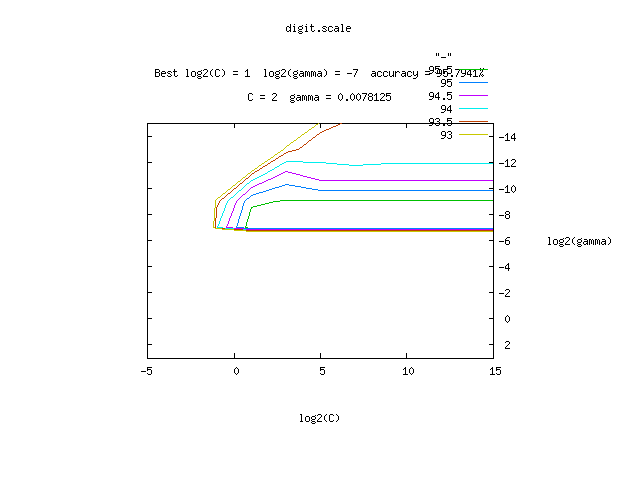
\includegraphics[width=1.0\textwidth]{digit}
\caption{grid search on $C,\gamma$}
\end{figure}

\section{Improvement}
\subsection{Motivation}
One observation from the algorithms is that neither decision tree nor SVM makes use of the information about the order of attributes. Actually, if some fixed permutation is applied on the attributes of each example in the data set, then decision tree and SVM will generate the same model as the model generated by original data set(subtle difference may exists, which depends on how the algorithm deals with ``tie conditions'', e.g. two attributes have the same information gain in C4.5). However, the positions of pixel are important for human when recognizing a image. Images also have strong 2-D local structure, pixels are correlated to pixels nearby\cite{lecun98}. If decision tree and SVM can make use of these information, their performance can be expected to have further improvement.\\

\subsection{Features Extraction}
One solution to this problem is to extract features which algorithms failed to capture. Feature extraction should be done before classification. In this paper, we extract several features derived from combination of pixels.\\
We add 16 extra features $r[16]$, one for each row, which describes how many ``black segments'' are there in the row. For example, in a image of ``1'', most of $r[i]$ can be expected to be $1$; in a image of ``0'', most $r[i]$ can be expected to be 2, and a few can be 1. Similarly, $c[16]$ are extracted for each column. The variance of the number of black pixels in each row and column are also added into each example.\\
Thus, 34 extra features are extracted. These features are appended after each instance. The modified data set has 290 features.
\subsection{Testing On Modified Data Set}
\vspace{0.5cm}
\begin{tabular}{c c c}
Algorithm		&	Original Data	&Modified Data\\
\hline \hline
C4.5                            &23.7916\%		& 18.5813\%\\
Pairwise C4.5                   &15.5345\%      & 12.3899\%\\
Boosted C4.5(32 iter)	        &7.7841\%		& 4.5198\%\\
Boosted PW C4.5(32 iter)	    &6.8553\%       & 5.2830\%\\
SVM                         	&4.2059\%       & 3.2643\%\\
\end{tabular}
\vspace{0.5cm}\\
From the result, we can see that all algorithms' error rates on modified data drop to some extent.\\
\subsection{Analysis}
By ranking the information gain of all attributes of the data set, in top 15 features, 14 of them are newly added features; 21 out of total 34 new features ranks less than 30. \\
In the decision tree of the new data set, new features are made heavily used of. The size of the new tree is 229, which is smaller than the size of the tree of the old data set(293 nodes). Since smaller trees tends to generalize better, C4.5 can have better performance on the modified data set.\\
SMO algorithm(in WEKA's implementation of SVM) gives 139 support vectors when trained by the whole original data set, while only 115 is obtained on the data set with new features. Although the number of features increases, the number of support vector decreases. The number of support vector can be seen as a measure of complexity of classifiers, thus SVM can have better performance on the new data set can be considered as the result of Occam's Razor principle.\\
\subsection{Testing on MNIST Data set}
MNIST(\url{http://yann.lecun.com/exdb/mnist/}) is a popular handwritten digit data set. This data set contains 60000 instances for training, and 10000 instances for testing.  Similar to Semeion data set, instances in MNIST data set consists of 28*28 pixels of a image, each pixel is described by the gray scale of the pixel. To make time cost feasible, we make a random sample of 1800 instances from the training set for training. The whole testing data set(10000 instance) is used for testing. This is because testing is relatively fast compared to training, and large testing set would give closer estimation to the real accuracy. The range of feature in the original data set is 0 to 256, which is too large. We normalize attributes of instances to range from 0 to 1. This is to avoid attributes in greater numeric ranges dominate those in smaller numeric ranges. Another advantage is to avoid numerical difficulties when calculating vector inner product\cite{svm}. We do not need to normalize the Semeion data set because the range of features are between 0 and 1 initially. Grid search shows that $C=8, \gamma=0.0078125$ gives optimal(locally) performance.\\
\vspace{0.5cm}
\begin{tabular}{c c}
Data Set	& Error rate\\
\hline \hline
MNIST	                  & 6.4\%\\
MNIST(extra features)	  & 5.72\%\\
\end{tabular}
\vspace{0.5cm}\\
The error rate reduces as expected when adding extra features. Thus feature extraction can be expected to work on general image classification problems.

\section{Further Work}
\begin{itemize}
 \item How Pairwise C4.5 performs on other multi-class classification problems compared to normal C4.5.
 \item Apply other method to build multi-class C4.5 from binary C4.5(e.g. one-versus-all).
 \item Find out more methods to extract features from image(e.g. corner, edge detection).
 \item Whether feature extraction can improve performance of other classification algorithms.
 \item Study classification algorithms which can automatically extract features of correlation of pixels(e.g. convolutional neural network\cite{lecun98}).
\end{itemize}
\section{Discussion}
This paper only discussed handwritten digit recognition, but methods mentioned in this paper also applies to other handwriting recognition problems in similar way.\\
Although feature extraction can improve classification performance, it can only extract small amount of information about pixel alignment and correlation data set. \\
We only test feature extraction on C4.5 and SVM. The effect on other algorithms are yet to be studied.\\

\section{Conclusion}
Comparing performance of different algorithms on on Semeion Data Set, C4.5 algorithm performs poorly, and adjusting parameters doesn't change the result much. Pairwise C4.5 performs better than C4.5. Boosted C4.5 and Boosted Pairwise C4.5 has a much better performance than C4.5. C-SVM with RBF kernel manages to reach 4.2059\% error rate after parameter search. By adding extracted features into the data set, the accuracy of all these algorithms improves, and SVM achieves the lowest error rate: 3.2643\%. Improvement of SVM is also observed on MNIST data set. Feature extraction can be expected to generalize on other image classification problems.

\newpage
\bibliographystyle{plain}
\bibliography{ref}
\end{document}
